\chapter{Background}
\label{sec:background}

Before going further in the implemented solutions, it's better to introduce a few background concepts. In particular, concepts about how FPGAs works, what kind of radiations exists and how FPGAs are affected by them.  

\section{Hardware Technology}

\subsection{FPGA Architecture}
\label{sec:fpgaarchitecture}
\textit{FPGAs} (Field Programmable Gate Arrays) are used in a wide range of applications, from signal processing to machine learning applications. In particular, it is an integrated circuit designed to be general purpose: after manufacturing, it has no funcionalities. It is a hardware that can be programmed to perform specific tasks. \bigskip

It differs from a CPU. A CPU is an already designed hardware that is designed to do only one thing in a very optimized way: execute code, from a pre-defined Instruction Set. In this case, the action of \textit{programming} is referred to the process of writing a series of instructions that the CPU will eventually execute. This is done by exploiting Programming Languges. A FPGA, instead, is like LEGO bricks. Each LEGO brick alone does not have any function or purpose, but when assembled (so put together with other bricks), it can be used to perform a specific task. Here, the action of \textit{programming} is referred to the process of writing a \textit{description} on how all the bricks will be assembled to perform the specific task we want. The description is done exploiting Hardware Description Languages (HDL) like VHDL or Verilog. \bigskip

The basic FPGA design conists of I/O pads (to connect with the outside world), a set of routing channels and a set of LEGO bricks. A LEGO brick in the FPGA is a logic block (and depending on the vendor, it can be called CLB or LAB) that can be programmed to perform a very specific task that in the overall design helps in achieving the goal of the User's Application. 

\begin{figure}[H]
\centering
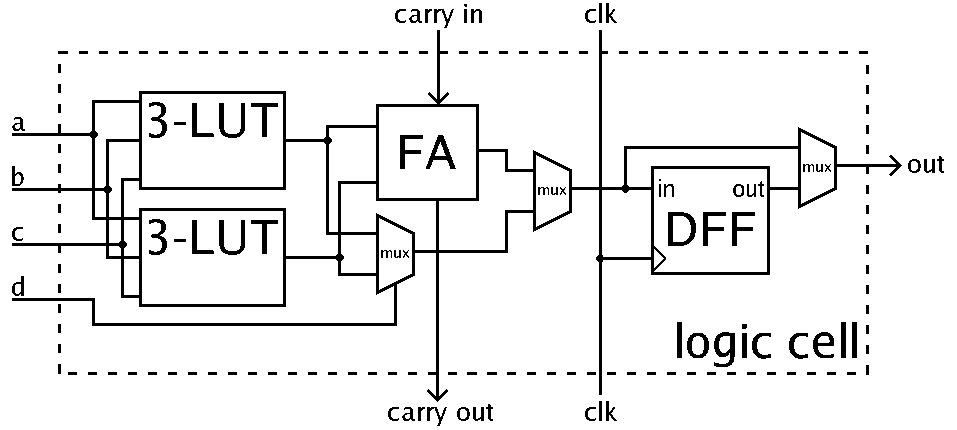
\includegraphics[width=1.0\linewidth]{images/chapter2/FPGA_cell_example.png}
\caption{Simplified schematic of a FPGA cell}
\label{fig:fpga_cell}
\end{figure}

A basic logic block consists of a few Logic Elements. As shown in figure \ref{fig:fpga_cell}, a Logic Elements is made of LUTs, a Full-Adder (FA), a D-Type Flip Flop and a bunch of multiplexers. This particular architecture can work in two modes: \textit{normal} mode and \textit{arithmetic} mode. Thanks to the Flip Flop, FPGAs can implement operations where some kind of memory is required.\bigskip

Modern FPGAs are very complex and expand upon the above capabilities to include other functionalities in silicon. Having these common functions embedded in the circuit reduces the area required and gives those functions increased speed compared to building them from logical primitives (because are implemented in-silicon, built out of transistor instead of LUTs, so they have ASICs-level performance). Examples of these include multipliers, generic DSP blocks, embedded processors, high speed I/O logic (like PCI/PCI-Express controllers, DRAM Controllers and so on and so forth) and embedded memories. \bigskip

Once the User's Application is designed (i.e. the description of the FPGA is written), the design needs to be mapped onto the FPGA's hardware resources. This is done using the Vendor's specific software and it's in charge of deciding which FPGA's LE is assigned to which subpart of the description and how each LE is configured. Then, all the LEs needs to be connected between themselfs and the I/O pads, and this is done by routing algorithms that decides the best way to connect them. Once all the implementation steps are done, a configuration file is generated that will eventually used to program the FPGA and is called \textit{bitstream}.\bigskip

All the programmable bits (like the content of the LUTs, some multiplexers selection signals or the routing details) are stored in the FPGA in memory elements that are outside the FPGA's funcional blocks (i.e. the one that can be used by the user to implement the application). Those memory elements can be though of as a big array of bits, or a \textit{shift register}. It's the \textit{configuration memory}: it stores the configuration bits of the entire FPGA and is loaded with the bitstream when the FPGA itself is programmed. Most FPGAs rely on an SRAM-based approach to be programmed: this allows to be in-system programmable (so the FPGA chip can be programmed without unmounting it from the board and from the system itself) and re-programmable (can be programmed as many times we want), but require external boot devices. Because the SRAM is a volatile memory, when the FPGA is powered off, the configuration memory content is lost. An external memory where the bitstream can be retrieved is required in order to re-program it. The SRAM approach is based on CMOS.\bigskip

Consequently, FPGAs are alternatives to hard-core CPUs. This means that on a FPGA a CPU can be implemented out of logic primitives (called \textit{soft-core}), alongside with the hardware that is used to implement the application like peripherals, memory and other components. Modern FPGAs supports \textit{at runtime programming}, this lead to the idea of \textit{reconfigurable systems}, where for example a CPU can be reconfigured in order to enable/disable some of its functionalities to suit the task at hand. The concept of \textit{reconfigurable systems} is also used in another manner and will be explained further in the next chapters.

\subsection{FPGAs vs. ASICs}

An \textit{ASIC} (application-specific integrated circuit) is an integrated circuit chip customized for a particular use. ASIC chips are typically fabricated using metal-oxide-semiconductor (MOS) technology. Thanks to the miniaturization of the MOS-based transistors and the improvement in the design tools, the maximum complexity (and hence functionality) possible in an ASIC has grown from 5000 logic gates to over 100 million. \bigskip

They are designed using the same HDLs Languages as the FPGAs, but the similarities stop there. Once the description is complete, specific ASIC softwares are used to synthesize and implement onto a technology library. While the corresponding technology library in FPGAs is simpler (made of LEs and routing elements), on ASICs it's a lot more complex. A typical ASIC technology library consists of a set of basic logic gates (like 2 input NAND, 3 input OR, 2 input FA, etc.) provided by the manufacturer that will manufactur the chip. Once a HDL description is mapped on top of the ASIC library, the so called \textit{gate-level netlist} is sent to the manufacturer. Here, ad-hoc technicians will start to work on this netlist, doing the \textit{route} {\&} \textit{place} of the netlist and as output of this process, a set of masks will be generated. The masks are used to \textit{print} the circuit in the silicon. On top of all this process, tests engineers must prepare a set of tests that in order to test the correct functionalities of the circuit during the various stages of the manufacturing process, until the end of the process itself. \bigskip

This allows to implement entire microprocessors, memories (including ROM, RAM, EEPROM and flash) and other large component in a single chip. Usually, for lower production volumes, FPGAs may be more cost-effective than an ASIC design. This is due to the non-recurring engineering (NRE) cost of an ASIC, that can run into millions of dollars. \bigskip

To recap:
\begin{itemize}
    \item ASICs circuits are faster, less power-hungry than FPGAs.
    \item ASICs are more complex to design and implement (hence more expensive) than FPGAs.
    \item FPGAs are more flexibile than ASICs.
\end{itemize}


\subsection{FPGA or ASIC in Aerospace Applications?}

In the aerospace industry, we are witnessing a turnaround in the last years regarding the hardware technology. FPGAs are typically much less radiation hardened than ASICs, so they are more prone to SEUs as well as lower total ionizing dose tolerance, but there are techniques to reduce these deficiencies. However, FPGAs are used on a lot more missions nowadays than 15 years ago, for all the reasons that make FPGAs a better choice than ASICs.\bigskip

As an example, Mars Exploration Rovers were something like 90\% ASICS. The last JPL's Martian Rover, Perserverance, is a very complex system and it's a very challenging design from the engineering point of view: it has multiple sensors and cameras to collect as much data as possible and, due to the volume of live data being recorded and the long data transmission time from Mars to Earth, a powerful processing system is essential. Early Mars rovers were basing their workload mainly on CPUs and ASICs as the processing units, while nowadays FPGAs are taking on much of the workload, like in Perseverance.\bigskip

There are different reasons behind this choice. The first one is the flexibility given by their re-programmability: because of the different stages a mission is made of, some parts of the system could be useful only in some of those stages (maybe intermediate ones) and they will never be used again. This is a waste of resources: FPGAs can be a great help in this aspect and Perserverance rover is an example. It utilizes an almost decade-old FPGA technology (Xilinx Virtex-5, introduced in May 2006 on 65 nm technology) as one of the main processing units. This unit is responsible for rover entry, descent and landing on Mars. Once the rover is landed, this unit would be useless and would become a \textit{dead hardware}. However, it's based on a FPGA hardware so it has been reprogrammed by NASA engineers from Earth to handle computer vision tasks.\bigskip

Other units on Perseverance such as radars, cameras, UHF transceivers, radar, and X-ray (used to identify chemicals) are controlled using Xilinx's FPGAs. Another interesting point is that Perserverance uses machine learning algorithm running on FPGAs, and they are so well optimized that it's achieving higher performance levels (about 18 times) than Curiosity rover (landed on Mars in 2012 and still active). \bigskip

Another advantage of using FPGAs is the faster time-to-space. There are different points that help in achieving this advantage. Not only the development on FPGA is faster than on ASICs (cost of design, development and fabrication of an ASIC are not present), but the most important thing is that there are many and many changes in the processing unit's architecture during project's development phase. There is usually a very stricted launch window for the mission that can be missed, and FPGAs help in two ways mainly:

\begin{itemize}
    \item Physically changing or adding more to a space system is a real challenge. The installation itself is not that difficult, but the system has to be recertified, proving that the it is still dependable. Furthermore, FPGAs simplify this greatly: the only thing to prove is that the FPGA chip is safe to fly with. Once this is done, the overall number of different parts to be certificied is reduced. Second, a change of the bitstream or of the software running on a \textit{soft-core} take a lot less time to certify.
    \item Software and Hardware development can be done in parallel. This is a great advantage for the software development team, because a first iteration of the hardware can be prepared and ready to use be used by the software team faster and the software team can start to work on the software itself.
\end{itemize}

FPGAs are not only helpful during the development phase, but even during the operational phase. Missions are prepared to last a relatively long time, but usually the quality of the work is so high that they last much longer. Examples are Mars rovers: Opportunity landed on the Red Planet in 2003 and it was ended by a martian dust storm in 2018, so it lasted for 15 years. Curiosity in 2012 and in 2022 is still active. This is a so long period that, speaking again about \textit{re-programmibility}, the processing system architecture may require changes to let the mission continue working. In fact, different things can go wrong in a decade and having a full reconfigurable system (from remote in particular) is a must, giving ground engineers a lot more possibilities to fix the system or to add/remove components. \bigskip

On the radiation tolerant side, vendors offer radiation-tolerant FPGAs. On top of that, it's possible to apply some logic changes to the design like TMR (Triple Module Redundacy) to a portion of the design or even to the entire design. Basically, it consists in triplicating the design and add a voter at the outputs. If a radiation error occurs, it will theoretically affect only one module so there will be two different results from the three modules (two correct and one wrong caused by the radiation). The voter will select the correct result (that is the majority). This is an example of making a design more robust to radiation.\bigskip

\section{Radiations}

We are going to understand better why radiation effects regarding electronic devices are one of the primary concerns for the aerospace industry.\bigskip

\subsection{Radiation sources}
Where does the radiation originate from? Unfortunately, the Universe and in particular the Solar System are full of radiations. The natural space radiation environment can damage electronic devices in different ways, ranging from a degradation in performances to a complete functional failure. More and more a space system goes deeper in the space, less and less it is protected by the Earth's atmosphere.\bigskip

Close to the Earth, there are two three sources of radiation: the Van Allen Belts, the Sun and the Cosmos itself. Van Allen Belts are zones of energetic charged particles, that are generated for example by the Sun, and captured by the Earth's magnetosphere. By trapping those charged particles, the magnetic field deflects them and protects the atmosphere from destruction. The two Earth's main belts extends from an altitude of 640 km to 58.000 km, in which radiation levels vary. Between the two belts, the \textit{inner} and the \textit{outer} there is a zone called \textit{safe zone} where the level of radiation is pretty low. Spacecrafts travelling beyond the LEO (Low Earth Orbit) go through the two belts, and beyond the belts they face additional hazards from cosmic rays and solar particle events (coronal mass ejections and solar flares).


\subsection{Radiation problems on Earth: the Nintendo's Super Mario 64 glitch}

Here on Earth, electronic devices are often not shielded or design to tolerate radiations. Usually, only safety-critical systems undergo the same kind of radiation-tolerant techniques as the ones used in the space system, like Aviation and Nuclear Power Plants, for instance.\bigskip

Even if there is a big magnetosphere protecting the planet's surface, some charged particles still escape and travel until they reach the ground and some everyday device. In 2013, a player was challenging another player in Nintendo's Super Mario 64 game. Suddenly, Mario was teleported into the air, saving crucial time and providing an incredible advantage in the game. The glitch caused the attention of a lot of players, and a \$1000 reweard was offered to anynone who could replicate the glitch. Users tried in vain to recreate the scenario, but no-one was able to emulate that giant leap. In the end, after eight years, user concluded that the glitch was not replicable because it was caused by a charged particle coming from the outer space that caused a bit-flip in the value that defines the player's height. \bigskip

Another curious case was the one related to the electronic voting machine in Belgium in 2003. A bit-flip here caused an adding of 4096 extra votes to a candidate. The error was only detected because there were more preferential votes than the candidate's own list, which is impossible in the voting system. The official explanation was ``the spontaneous creation of a bit at the position 13 in the memory of the computer''. It's not a coincidence that the value added was exactly 4096, in hexadecimal \texttt{0x1000}, that is $2^{12}$.

\subsection{Types of radiation}
The most common way to classify radiations is based on their effects on electronic devices. If the effect is the result of a cumulative damage (i.e. passage of many charged particles in different moments in time, and each particle has a relative low energy) then it can be a \textit{total ionizing dose} or a \textit{displacement ionizing dose}. If the effect is the result of a single charged particle (with a high energy) then it can be \textit{destructive} or \textit{non-destructive}, and they are usually referred as SEE (Single Event Effects). \bigskip

\subsubsection{Total ionizing dose}
Most electronic devices are based on MOS transistors, forming the basis for digital logic. The common way to use those transistors is as \textit{electronic switches}: there are two isolated contacts, the source and the drain (i.e. the switch is off, no current). When a positive charge is applied to the gate (in the case of a NMOS transistor), electrons (that are negative charges) are allowed to pass from the two isolated contacts (i.e. the switch is on). \bigskip

When ionizing radiations passes through the device, electrons are moved away from the material leaving 
``holes'' of missing charge, acting as positive charge carriers. These holes can find their way to the gate oxide and become trapped: this phenomenon is called \textit{total ionizing dose}. The effect of this phenomenon is the same as applying some positive voltage to the gate. With enough accumulated charges, the effect is to have the transistor always on, or better, in the \textit{stuck-on state}. \bigskip

\subsubsection{Displacement ionizing dose}
Another form of cumulative damage is the \textit{displacement ionizing dose}. This is the effect of a single charged particle passing through the device. What happens is that an atom is displaced from the material, modifying the crystal structure of the material itself. These microscopic effects create traps and recombination centers, eventually leading to the modification of the free flow of the current. This will ultimately impact the device's performance. \bigskip

\subsection{Single Event Effects}
When a single high-energy charged particle passes through the device, it can cause a \textit{destructive} or \textit{non-destructive} effect. The particle creates a momentary change of charge in the device, creating an unexpected current that can affect the device in various ways. Some effects may be completely destructive, while others may degrade performance to the point that the device doesn't work anymore in the limits required by the circuit or the system itself. Other effects cause the device to momentarily work in a wrong way, causing a functional failure (so it's not destructive from the point of view of the device but can cause an functional error, for example a wrong value in the memory from \textit{0xe} to \textit{0xf}). \bigskip

Within the destructive effect, the most common are Single Event Latchup (SEL), Single Event Burnout (SEB) and Single Event Gate Rupture (SEGR).

\subsubsection{Single Event Latchup}
In CMOS technology, there are a lot of intrinsic BJT (Bipolar Junction Transistor). When a special arrangement of PMOS and NMOS transistors is used, resulting in a n-p-n-p structures (corresponding to a NPN and a PNP transistor stucked next to each other), a CMOS Latchup structure is created. If one of these two transistor is activated (accidentally by a high-energy charged particle), the other one will be activated too, creating a feedback loop. They will both keep each other activated for a long as some current flows through them. This phenomenon will increase the current draw and can bring to the destrupution of the device. Usually, the only way to correct this situation is to make a \textit{power cycle}, so completely shutting down the device and then restarting it. However, latent damage may exists that may not appear until later. \bigskip

\begin{figure}[H]
\centering
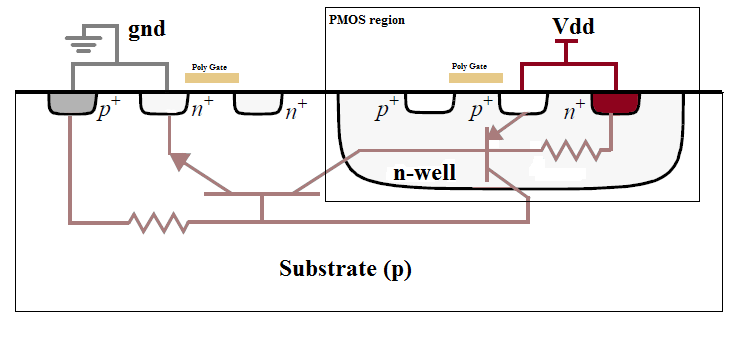
\includegraphics[width=1.0\linewidth]{images/chapter2/Latchup.png}
\caption{The intrisic BJTs in the CMOS Technology that can cause a Latchup. Deepon, CC BY-SA 3.0, via Wikimedia Commons}
\label{fig:latchup}
\end{figure}

\subsubsection{Single Event Burnout}
Can happen when an incident particle initiates an avalanche charge multiplication effect. This leads to an increasing current, leading to a thermal runaway of the device, causing local melting or ejection of molten material in a small-scale explosion. Obviously, the result is a complete destruction of the device. \bigskip

\subsubsection{Single Event Gate Rupture}
SEGR is the destructive rupture of a gate oxide (or any dielectric layer in a transistor). The effects can be observed in power MOSFETs with an increase of current flow when turned on, or in digital circuits with stuck bits. 

\subsubsection{Single Event Upset}
This is the most common non-destructive effect. As known as \textit{bit-flip}, it's caused by a particle that forces a digital signal to an opposite value momentarily. It can lean in a temporary modification of the digital output in a combinatory circuit, and the modified value can be memorized in a flip-flop or any other memory element if sampled at the same time a radiation arrives. In more complex circuits, it can cause other malfunctions like resets and memory values modifications. \bigskip

\begin{figure}[H]
\centering
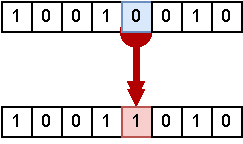
\includegraphics[height=0.2\linewidth]{images/chapter2/SEU_EXAMPLE.pdf}
\caption{Example of a Single Event Upset in a memory element.}
\label{fig:seu_example}
\end{figure}

What is shown in Figure \ref{fig:seu_example} can for example happen in a SRAM memory. Each cell is made of a cross-coupled transistors. Each side couple are connected forming an inverter (NOT logic function), and the output of the inverter is connected to the gates of the second couple.  

\begin{figure}[H]
\centering
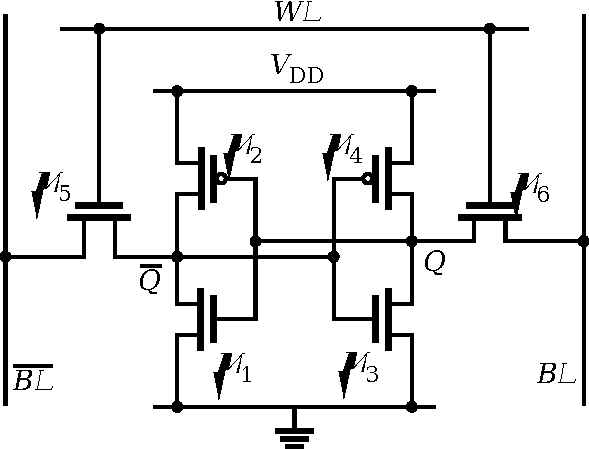
\includegraphics[height=0.4\linewidth]{images/chapter2/SRAM_CELL.pdf}
\caption{Simple SRAM Cell layout. Inductiveload, Public domain, via Wikimedia Commons.}
\label{fig:sram_cell_layout}
\end{figure}

In Figure \ref{fig:sram_cell_layout}, a simple layout is proposed. In order to have a logic 0 as output (\textit{BL = 0}), M3 is active (thus M4 is not active). So M2 is active (thus M3 is not active). If a radiation strikes one of those transistor, can happen that the M3's gate voltage goes low, causing a flip of the configuration thus a flip of the stored bit. \bigskip

As explained in Section \ref{sec:fpgaarchitecture}, most FPGAs' memory configuration are based on SRAM technology. If a bitflip occurs, the FPGA configuration itself is modified, leading to a malfunction of a module or to a routing modification.\bigskip

% Explain why the trends (smaller transistors) cause SEU to be more common than accumulation effects.